\chapter{Grundlagen}
Dieses Kapitel verschafft einen Überblick über die benötigten theoretische Grundlagen, um die Methoden dieser Arbeit zu verstehen. 
Zunächst wird eine Einführung in Neuronale Netzwerke gegeben, anschließend werden
einzelne Bestandsteile und Varianten von Neuronalen Netzwerken erklärt. 
Als nächstes werden der ``Lab-Farbraum'' und die Image Colorization Methoden kurz erläutert. Abschließend wird ein Überblick über verwandte Arbeiten gegeben.

\section{Neuronale Netze}
Künstliche Neuronale Netze sind vom menschlichen Gehirn inspiriert und werden für Künstliche Intelligenz und Maschinelles Lernen
angewendet. Genutzt werden sie für überwachtes und unüberwachtes lernen. In der vorliegenden Arbeit werden nur Methoden des überwachten
lernens angewendet. Beim überwachten lernen sind die Datensätze gelabelt, sodass der Output des Neuronalen Netzes mit den richtigen Ergebnissen
verglichen werden kann.
\\
\\
Neuronale Netze bestehen aus Neuronen, auch ``Units'' genannt, die schichtenweise in ``Layers'' (Schichten) angeordnet sind.
Beginnend mit der Eingabeschicht (Input \gls{Layer}) fließen Informationen über eine oder mehrere Zwischenschichten (Hidden \gls{Layer}s) bis hin zur 
Ausgabeschicht (Output \gls{Layer}). Dabei ist der Output des einen Neurons der Input des nächsten. \cite{neuronale-netze-aufbau}

\subsection{Feedforward Neural Network}
Das Ziel von einem Feedforward Neural Network ist die Annäherung an eine Funktion $ f^* $. Ein Feedforward Neural Network definiert 
eine Abbildung $ y = f(x;W) $ wobei $ x $ der Input ist und $ W $ die lernbaren Parameter sind (auch Gewichte genannt).
\cite[164-223]{Goodfellow-et-al-2016}
\\
\\
Diese Netzwerkarchitektur trägt den Namen ``feedforward'' weil der Informationsfluss von dem Input \gls{Layer},
über die Hidden Layers bis zum Output \gls{Layer} in eine Richtung weitergereicht wird.

Feedforward Neural Networks werden als eine Kette von Funktionen dargestellt. So,
kann man die Funktionen $ f^{(1)}, f^{(2)}, f^{(3)} $ in Form einer Kette verbinden, um $ f(\textbf{x}) = f^{(3)}(f^{(2)}(f^{(1)}(\textbf{x}))) $
zu bekommen. Diese Kettenstrukturen sind die am häufigsten genutzte Struktur bei Neuronalen Netzwerken. Im genannten Beispiel ist $ f^{(1)} $ die
erste Layer, $ f^{(2)} $ die zweite und $ f^{(3)} $ die Output Layer von diesem Netzwerk. Die Länge dieser Kette definiert die Tiefe des Netzwerks.
Je tiefer ein Netzwerk ist, desto mehr erlernbare Parameter besitzt es und braucht somit eine erhöhte Rechenleistung, um trainiert zu werden.
In der Praxis sind die Netzwerke sehr tief, daher der Begriff Deep Learning.
\\
\\
Während dem Training werden die Gewichte von $ f(x) $ verstellt, um $ f^*(x) $ zu erhalten. Jedes Trainingsbeispiel $ x $ ist mit einem Label
$ y = f^*(x)$ versehen. Die Trainingsbeispiele geben genau vor, was die Output Layer generieren soll. Die Output Layer soll Werte generieren,
die nah an $ y $ liegen. Das Verhalten die Hidden Layers wird nicht durch die Trainingsbeispiele festgelegt, sondern der Lernalgorithmus
soll selbst definieren, wie diese Layers verwendet werden, um die beste Annäherung von $ f^*(x) $ zu erzielen.

\subsection{Fully-connected Neural Network}
Fully-connected Neural Networks sind die am häufigsten vorkommende Art von Neuronalen Netzen. In dieser Netzwerkarchitektur sind alle Neuronen
eines Layers mit allen Neuronen des vorherigen und des nächsten Layers verbunden. Neuronen die sich im selben Layer befinden, 
sind jedoch nicht miteinander verbunden.
\cite{cs231-neural-networks}

\begin{figure}[H]
  \centering
  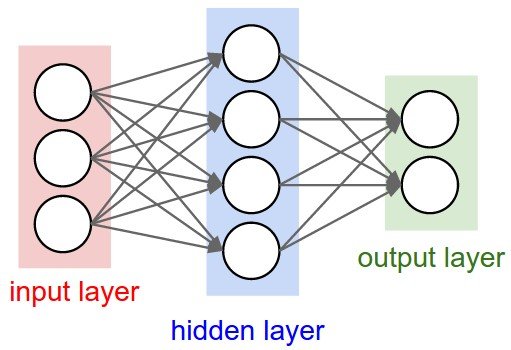
\includegraphics[width=0.65\textwidth]{resources/nn/neural_net.jpeg}
  \caption{
    Fully-connected Neural Network mit 2 Layers (eine Hidden Layer mit 4 Neuronen und eine Output Layer mit 2 Neuronen)
    \cite{fully-connected-neural-network}
  }
  \label{image:neuronal-network}
\end{figure}

Einer der wichtigsten Gründe für die Anordnung von Neuronalen Netzen in Layers ist, dass so eine Struktur anhand von Matrix Multiplikationen
berechnet werden kann. Die Abbildung \ref{image:neuronal-network} stellt ein Netzwerk mit 3 Inputs $ x $, einer Hidden Layer mit 4 Neuronen
und einer Output Layer mit 2 Neuronen dar. Die Kreise repräsentieren die Neuronen und einen Bias Wert $ b $,
die Pfeile stellen die Gewichte $ w $ dar.

\begin{align}
  f(x) = w*x + b
\end{align}

Nach jedem Hidden Layer läuft der Output durch eine Aktivierungsfunktion $ \sigma $ die unter Kapitel \ref{subsection:aktivierungsfunktionen} erklärt wird.
Dadurch wird die vorherige Formel um $ \sigma $ erweitert:

\begin{align}
  f(x) = \sigma( w*x + b)
\end{align}

\subsubsection{Forward Pass}
Der Forward Pass von einem Neuronalen Netz wird anhand von Matrizen Multiplikationen berechnet. Um dies zu veranschaulichen wird
es anhand eines Beispiels erklärt.

Ausgehend von einem Netzwerk mit 3 Inputs, einer Hidden Layer mit 2 Neuronen und einem Output Neuron, ergeben sich folgende Beispielwerte:
\begin{equation} 
  \vspace{5pt}
  X = \begin{pmatrix}
    1 &0 &1 &1 \\
    1 &1 &1 &0 \\
    1 &1 &0 &1
  \end{pmatrix} 
  \hspace{5pt}
  W = \begin{pmatrix}
    10 &20 \\
    -20 &-40 \\
    20 &0 \\
    -40 &0
  \end{pmatrix}
  \hspace{5pt}
  W_{out} = \begin{pmatrix}
    20 \\
    40 \\
    -40
  \end{pmatrix}
\end{equation}

$ X $ sind die Inputs, $ W $ die Gewichte des Hidden Layers und $ W_{out} $ die Gewichte des Output Layers.
Die erste Spalte aus dem Input $ X $ und die ersten Zeilen aus beide Gewichtsmatrizen $ W $ und $ W_{out} $ sind die Werte für den Bias.
Diese Anordnung des Bias Wertes ermöglicht die Berechnung durch eine einzige Matrix Multiplikation. Als Aktivierungsfunktion wird ReLU 
\cite{10.5555/3104322.3104425} verwendet:

\begin{equation}
  \vspace{5pt}
  f(x) = 
  \begin{cases}
    0 &\text{if \(x < 0\)}  \\
    x &\text{if \(x \geq 0\)} 
  \end{cases}
\end{equation}

Im ersten Schritt durchläuft der Input die Hidden Layer $ f(X \times W) $:
\begin{equation}
  \vspace{5pt}
  f \left(
  \begin{pmatrix}
    1 &0 &1 &1 \\
    1 &1 &1 &0 \\
    1 &1 &0 &1
  \end{pmatrix}
  \times
  \begin{pmatrix}
    10 &20 \\
    -20 &-40 \\
    20 &0 \\
    -40 &0
  \end{pmatrix}
  \right)
  =
  \begin{pmatrix}
    0 &1 \\
    1 &0 \\
    0 &0
  \end{pmatrix}
\end{equation}

Im zweiten Schritt wird der Output von der vorherigen Multiplikation mit den Gewichten des Output Layers multipliziert:
\begin{equation}
  \vspace{5pt}
  f \left(
  \begin{pmatrix}
    1 &0 &1 \\
    1 &1 &0 \\
    1 &0 &0
  \end{pmatrix}
  \times
  \begin{pmatrix}
    20 \\
    40 \\
    -40
  \end{pmatrix}
  \right)
  =
  \begin{pmatrix}
    0 \\
    1 \\
    0
  \end{pmatrix}
\end{equation}

\newpage
\subsection{Aktivierungsfunktionen}\label{subsection:aktivierungsfunktionen}
Eine Aktivierungsfunktion definiert die Aktivierungsrate von einem Neuron. Es gibt verschiedene Aktivierungsfunktionen:

\subsubsection{Sigmoid}
Sigmoid ist eine nicht lineare Funktion welche die Werte in einem Wertebereich von $ [0, 1] $ bringt.
Große negative Werte werden annähernd 0 und große positive Werte werden annähernd 1. Sigmoid hat einige Nachteile, so neigt es dazu den Gradienten
verschwinden zu lassen und die Outputs sind nicht Null zentriert. Sigmoid wird definiert als:

\begin{equation}
  \sigma(x) = \frac{1}{1 + e^{-x}}
\end{equation}

wobei $x$ ein Input ist.

\begin{figure}[H]
  \centering
  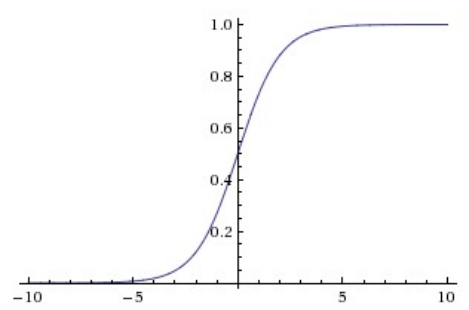
\includegraphics[width=0.5\textwidth]{resources/nn/sigmoid.png}
  \caption{
    Sigmoid Aktivierungsfunktion 
    \cite{neuron-model}
  }
  \label{image:sigmoid}
\end{figure}

\subsubsection{Tanh}
Die Tanh Aktivierungsfunktion bringt Werte in einen Wertebereich von $ [-1, 1] $. Es ist eine skalierte Sigmoid ($ \sigma $) Funktion,
$ tanh(x) = 2\sigma(2x) - 1 $. Die Nachteile von Tanh ähneln den von Sigmoid, wobei jedoch der Output Null zentriert ist.

\begin{figure}[H]
  \centering
  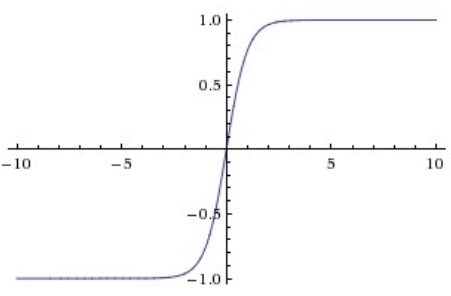
\includegraphics[width=0.5\textwidth]{resources/nn/tanh.png}
  \caption{
    Tanh Aktivierungsfunktion 
    \cite{neuron-model}
  }
  \label{image:tanh}
\end{figure}

\subsubsection{ReLU}
Die Rectified Linear Unit konvertiert alle negativen Werte zu 0 und alle positiven Werte behalten ihre Identität. Diese Aktivierungsfunktion
wurde für die Netzwerke in dieser Arbeit verwendet da, sie Vorteile gegenüber Sigmoid und Tanh zeigt. Einer der Vorteile ist, dass die mathematische
Auswertung der Funktion unkompliziert ist. Außerdem beschleunigt sie die Konvergenz des Stochastischen Gradientenabstiegsverfahrens im Vergleich zu Sigmoid.
ReLU ist definiert als:

\begin{equation}
  f(x) = max(0, x)
\end{equation}

wobei $x$ ein Input ist.
\\
Neuronen die ReLU als Aktivierungsfunktion verwenden können während des Trainings ``sterben''. Zum Beispiel, wenn der Gradient in einem Neuron
zu groß ist, kann dieser zu einem update der Gewichte führen, wodurch das Neuron nie wieder aktiviert werden kann. Mit einer korrekten Einstellung der
Lernrate kann das vermieden werden. \cite{cs231-neural-networks}

\begin{figure}[H]
  \centering
  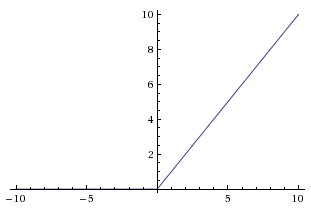
\includegraphics[width=0.5\textwidth]{resources/nn/relu.jpeg}
  \caption{
    Rectified Linear Unit (ReLU) 
    \cite{neuron-model}
  }
  \label{image:relu}
\end{figure}

\subsubsection{Leaky ReLU}
Leaky ReLU ist einer Variante der ReLU Aktivierungsfunktion, die versucht das Problem der ``sterbenden'' Neuronen zu minimieren. Anstatt alle negativen Werte
zu Null zu konvertieren, werden die Werte mit einer Konstanten multipliziert. Die Funktion wird zu $ f(x) = 1(x < 0)(\alpha x) + 1(x >= 0)(x)$,
wobei $ \alpha $ eine Konstante mit geringerem Wert ist, zum Beispiel $ 0.001 $.

\begin{figure}[H]
  \centering
  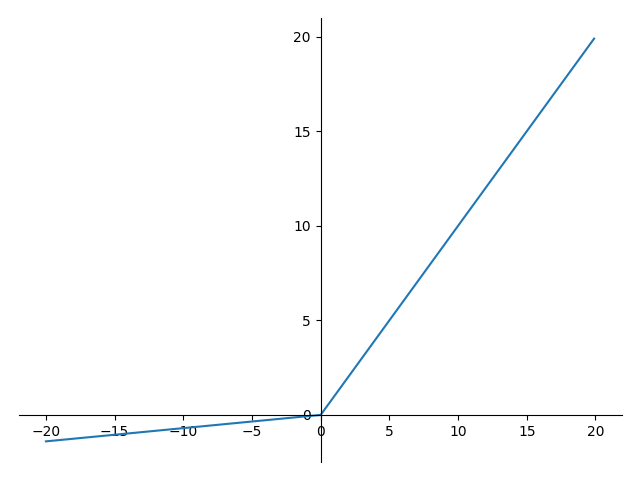
\includegraphics[width=0.5\textwidth]{resources/nn/leaky-relu.png}
  \caption{
    Leaky ReLU 
    \cite{leaky-relu}
  }
  \label{image:leaky-relu}
\end{figure}

\newpage
\subsection{Loss Functions}
% Erklärung
Die \gls{loss function} (Kostenfunktion) dient zur Feststellung der Fehler (Loss) zwischen dem Output von einem Modell und dem vorgesehenen Zielwerten. 
Das Ziel von Neuronalen Netzen ist es den Loss zu minimieren. Wenn der Loss gleich Null ist, heißt dass $ y = \hat{y} $. Es gibt verschiedene Arten 
von \gls{loss function}s. Im Rahmen dieser Arbeit werden \gls{loss function}s bezogen auf Regressions– und Klassifizierungsprobleme behandelt.

\subsubsection{Mean Square Error Loss}
Mean Square Error (MSE) Loss misst den mittleren quadratischen Fehler und ist definiert als:

\begin{equation}
  J = \frac{1}{N} \sum (y - \hat{y})^2
\end{equation}

wobei, $J$ der Loss ist, $N$ die Anzahl der Klassen, $y$ die korrekte Klasse (\gls{ground truth}) und $ \hat{y}$ die vorhergesagte Klasse ist.

\subsubsection{Cross Entropy Loss}
Der Cross Entropy Loss wird bei Klassifizierungsproblemen verwendet. Es wird unterschieden zwischen, Binär und Multiclass Cross Entropy Loss. 
Bei dem Multiclass Cross Entropy Loss wird ein Vektor mit einer Wahrscheinlichkeitsverteilung $ x \in [0, 1] $ 
ausgewertet, wenn die korrekte Klasse eine 1 besitzt ist der Loss 0. Dabei gilt: je weniger Wahrscheinlichkeit die korrekte Klasse besitzt, 
desto höher wird der Loss sein. Der Multiclass Cross Entropy Loss ist definiert als: 

\begin{equation}
  J = -\frac{1}{N} \Big(\sum_{i=0}^N y_{i} * \log(\hat{y_{i}})\Big)
\end{equation}

wobei, $J$ der Loss ist, $N$ die Anzahl der Klassen, $y$ die Korrekte Klasse (\gls{ground truth}) und $ \hat{y}$ die vorhergesagte Klasse.

\subsubsection{Weighted Cross Entropy Loss}
Bei dem Weighted Cross Entropy Loss werden die Klassen gewichtet bevor der Loss berechnet wird. Das ist zum Beispiel nützlich, um Klassen  
mit einer niedrigen Wahrscheinlichkeit zu bevorzugen.

\subsection{Optimierungsalgorithmen}
Das Ziel von Optimierungsalgorithmen ist eine Kombination von Gewichten $ W $ zu finden, die die \gls{loss function} minimieren.
Es gibt diverse relevante Optimierungsalgorithmen. In der vorliegenden Arbeit werden Gradient Descent, Adam und RMSProp verwendet.

% TODO: Erklärung für update rules anpassen
\subsubsection{Gradient Descent}
Gradient Descent (Gradientenabstiegsverfahren) ist ein iteratives Verfahren, um bei einer Funktion das Minimum (oder das Maximum) zu finden. 
Mit Hilfe von partiellen Ableitungen kann der Gradient von einer Funktion berechnet werden. Ein Gradient ist, im Fall von Neuronalen
Netzen, ein Vektor, der zum höchsten Punkt der \gls{loss function} zeigt. Wird der negative Gradient genommen, zeigt dieser zum tiefsten Punkt.
Bei jeder Kombination von Gewichten wird der Gradient berechnet und mit einer bestimmten Lernrate $ \alpha $ multipliziert, anschließend werden 
alle Gewichte aktualisiert. Die Lernrate definiert die Größe der Schritte in Richtung Minimum. Die Update Regel für die Gewichte ist definiert als:

\begin{equation}
  w_{x+1} = w_x - \alpha * \nabla J(w_x)
\end{equation}

wobei, $w_{x+1}$ die aktualisierten Gewichte sind, $w_x$ die vorherigen Gewichte, $ \alpha $ die Lernrate und $\nabla J(w_x)$ der Gradient. 
Die Update Regel für den Bias sieht identisch aus.

\begin{figure}[H]
  \centering
  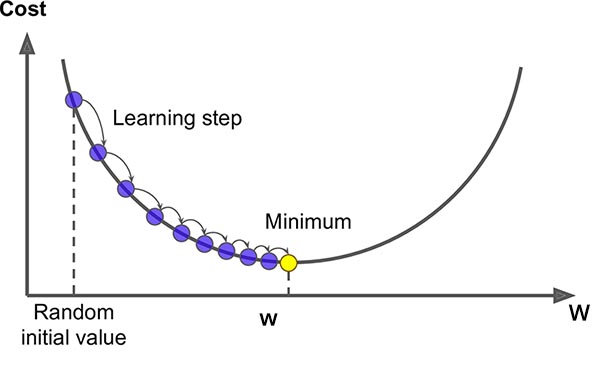
\includegraphics[width=0.65\textwidth]{resources/cnn/gradient-descent.jpg}
  \caption{
    Gradient descent visualisiert
    \cite{gradient-descent}
  }
  \label{image:gradient-descent}
\end{figure}

Es gibt verschiedene Arten von Gradient Descent: Gradient Descent, Mini-Batch Gradient Descent und Stochastic Gradient Descent. 
Beim Gradient Descent
werden die Gradienten im Bezug zu dem gesamten Datensatz berechnet und damit das Update durchgeführt. Der Mini-Batch Gradient Descent berechnet 
die Gradienten im Bezug zu einem kleinen Teil des Datensatzes und führt ein Update für alle Parameter durch. Der Stochastic Gradient Descent 
berechnet den Gradient bezogen auf ein einziges Element des Datensatzes und führt einen Update für alle Parameter durch.
\\
Um die Konvergenz Richtung Minimum zu beschleunigen wurde der Gradient Descent mit Momentum entwickelt. Bei diesem Ansatz wird ein
Geschwindigkeitsparameter zu der Update Regel hinzugefügt, der alle vorherigen Updates akkumuliert. 
Das ermöglicht die schnellere Konvergenz mit jedem Schritt. Die neue Update Regel ist definiert als:

\begin{equation}
  \begin{gathered}
    v_{t+1} = \rho v_t - \alpha * \nabla J(w_x) \\
    w_{x+1} = w_x + v_{t+1}
  \end{gathered}
\end{equation}

wobei $v_{t+1}$ der nächste Geschwindigkeitsparameter ist, $v_t$ der aktuelle Geschwindigkeitsparameter und $\rho$ ein Reibungsparameter 
(typisch 0.9) zur Regulierung.

% TODO: finish Adam
\subsubsection{Adam}
Adam steht für ``Adaptive Moment Estimation Algorithm'' und ist ein Optimierungsalgorithmus, der eine angepasste Lernrate für die verschiedenen
Parameter berechnet \cite{kingma2014adam} zusätzlich zu der Speicherung des exponentiell abnehmenden Mittelwerts vorangegangener Gradienten.
Adam ist der bevorzugte Optimierungsalgorithmus für die vorliegende Arbeit. 
Adam kombiniert die Ansätze von AdaGrad \cite{duchi2011adaptive} und RMSProp. AdaGrad ist eine 
verbesserte Version von Gradient Descent, der eine angepasste Lernrate für die verschiedenen Parameter einführt. 

\subsection{Backpropagation}\label{subsection:backpropagation}
Neuronale Netze lernen indem der Loss minimiert wird. Wie in der vorherigen Sektionen erläutert, bestimmt die \gls{loss function}
die Fehlerrate von einem Neuronalen Netz. Dieser Loss kann mit Hilfe von einem Optimierungsalgorithmus reduziert werden. 
Backpropagation ermöglicht eine effiziente Berechnung der Gradienten in einem neuronalen Netzwerk \cite{was-ist-backpropagation}. 
Mit Hilfe der Kettenregel kann eine komplexe \gls{loss function} in kleinere Unterfunktionen zerlegt werden, um Lokal die Ableitung zu berechnen.
Das ermöglicht eine unkomplizierte Berechnung des Gradienten.
\\
\\
Als Beispiel wird die folgende Sigmoid Funktion in Unterfunktionen zerlegt:

\begin{equation}
  f(w,x) = \frac{1}{1+e^{-(w_0 x_0 + w_1 x_1 + w_2)}}
\end{equation}

\begin{figure}[H]
  \centering
  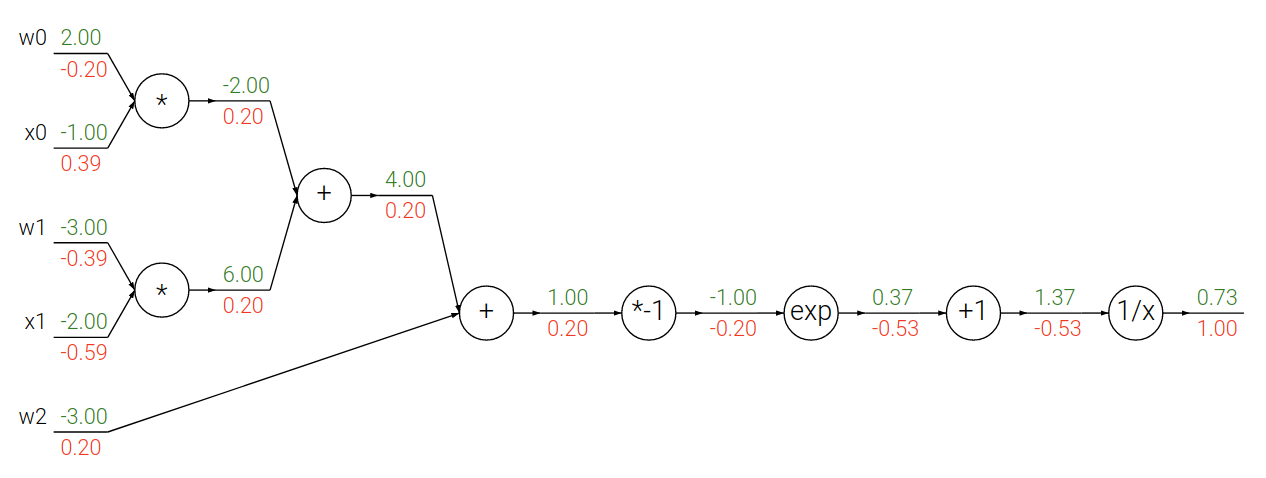
\includegraphics[width=1\textwidth]{resources/cnn/backpropagation.png}
  \caption{
    Backpropagation Beispiel anhand einer 2D Neuron mit der Aktivierungsfunktion Sigmoid
    \cite{backpropagation}
  }
  \label{image:backpropagation}
\end{figure}

Auf der Abbildung \ref{image:backpropagation} stellen $ [w_0, w_1, w_2] $ die Gewichte und $ [x_0, x_1] $ die Inputs des Neurons dar. 
Um es unkompliziert zu halten wird die 
obere Funktion als eine beliebige Funktion, die Inputs ($w, x$) entgegennimmt und eine einzelne Zahl als Output hat, visualisiert werden. 
Die grünen Zahlen repräsentieren die Ergebnissen aus dem Forward Pass und die roten Zahlen den zurück propagierten Loss. Jeder Knoten ist fähig 
ein Output und der lokale Gradient von dem Output im Bezug auf den Input zu berechnen, ohne die komplette Funktion kennen zu müssen \cite{cs231-backpropagation}.

\section{Convolutional Neural Networks}
Convolutional Neural Networks (\gls{CNN}) sind eine besondere Form von künstlichen neuronalen Netzwerken, die unter anderen speziell für 
die Verarbeitung von Bilddaten, vorgesehen sind \cite{convnet-erklaerung}.
\\
Im Gegensatz zu traditionellen neuronalen Netzwerken, die einen Vektor als Input nehmen, nehmen Convolutional Neural Networks ein 3D Volumen als Input
($ W \times H \times C $, hierbei ist $W$ die Breite, $H$ die Höhe und $C$ sind die Farbkanäle).

\begin{figure}[H]
  \centering
  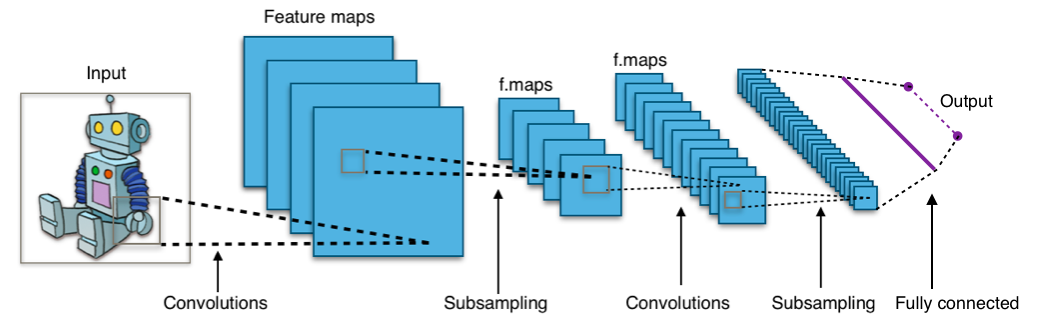
\includegraphics[width=1\textwidth]{resources/cnn/typical_cnn.png}
  \caption{
    Typische Struktur von einem Convolutional Neural Network
    \cite{typical_cnn_img}
  }
  \label{image:typical_cnn_img}
\end{figure}


\gls{CNN}s bestehen in der Regel aus 2 Formen von \gls{Layer}s, der Convolutional \gls{Layer} und der Pooling Layer. 
\\
\\
Die Convolutional \gls{Layer} besteht aus mehreren hintereinander geschalteten 3 dimensionalen
Filtern, auch Kernel genannt ($ W \times H \times D$, wobei $D$ die Tiefe der Feature Maps darstellt), die während dem Forward pass mit 
einer festgelegten Schrittweite (\gls{stride}), über das Bild geschoben werden. Mit dem sogenannten Padding wird das Verhalten an den Rändern festgelegt.
An jeder Stelle wird eine Matrix Multiplikation zwischen den Filter und die aktuelle Position auf dem Bild durchgeführt. 
Als Output wird eine 2 dimensionalen Feature Map generiert. Die Größe dieser Feature Map ist abhängig 
von der Größe des Filters, dem Padding und vor allem dem \gls{stride}. Ein \gls{stride} von 2 bei einer Filter Größe von $ 2\times2 $ führt beispielsweise 
pro Filter zu einer Halbierung der Größe der Feature Map im Vergleich zum Input Volumen \cite{aufbau-funktion-convnet}.
Ein \gls{stride} von 1 bei einem $ 3\times3 $ Filter mit Padding 1 führt zu einer Feature Map mit der gleiche Größe wie dem Input Volumen.
\\
\\
Die Filter erkennen in den ersten Ebenen einfache Strukturen wie Linien, Farben oder Kanten. In den daran folgenden Ebenen lernt das CNN Kombinationen aus 
diesen Strukturen wie Formen oder Kurven. In den tieferen \gls{Layer}s werden komplexere Strukturen und Objekte identifiziert. 

\begin{figure}[H]
  \centering
  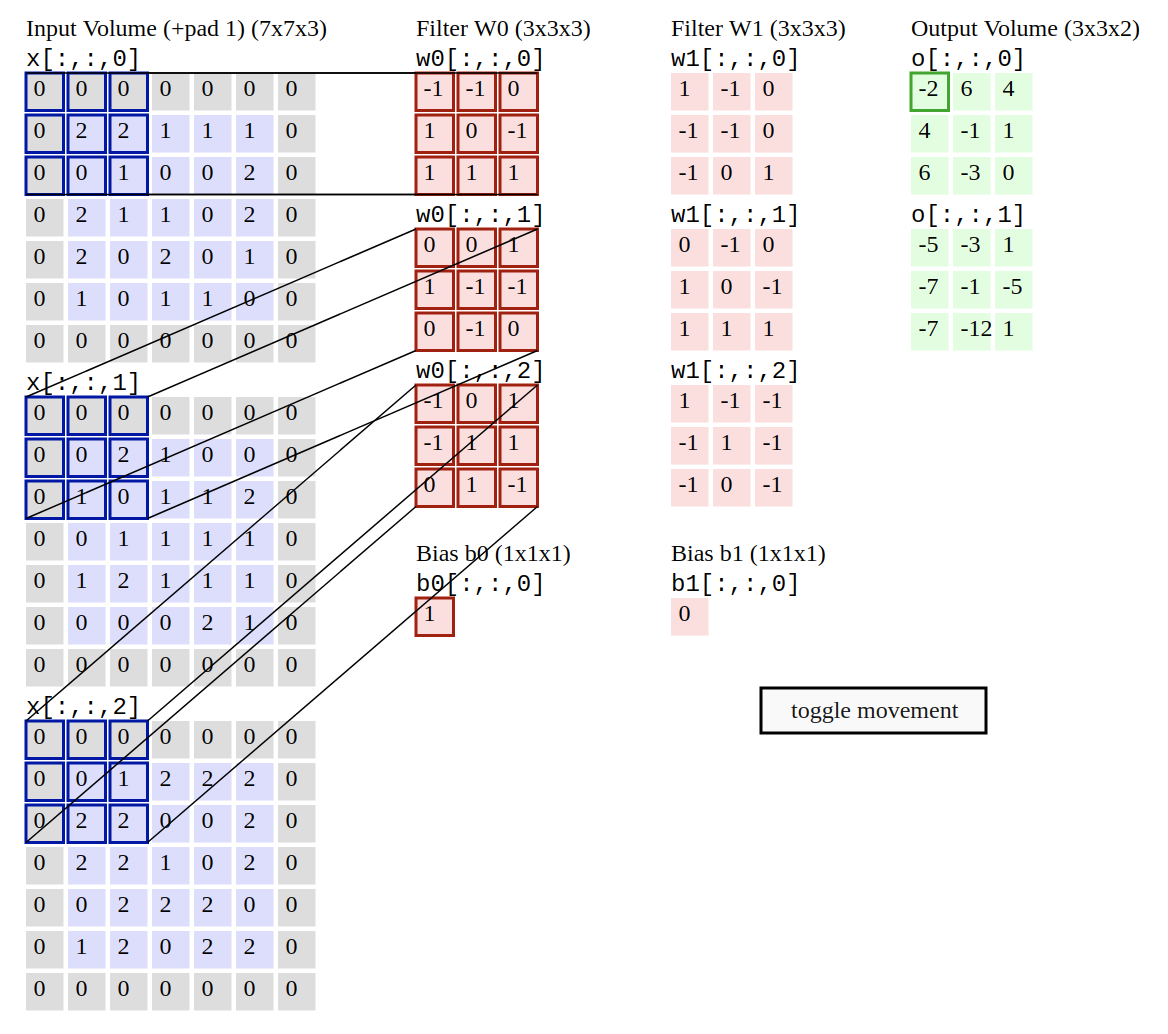
\includegraphics[width=0.75\textwidth]{resources/cnn/funktion-cnn.png}
  \caption{
    Beispiel eines Forward pass von einer Convolutional \gls{Layer} mit einem $ 7\times7\times3 $ Input Volumen, zwei $3\times3\times3$ Filtern, 
    Padding 1 und \gls{stride} 2.
    \cite{convnet-demo}
  }
  \label{image:convnet-demo}
\end{figure}

Die Pooling Layer dient zur Reduktion der Dimensionen von einem Input Volumen und somit den Parametern vom Netzwerk. Es gibt 
verschiedene Pooling Operationen die angewendet werden können, wie zum Beispiel Maximum Pooling, Minimum Pooling, oder Average Pooling. Im Rahmen 
dieser Arbeit wird Maximum Pooling (auch Max Pooling genannt) verwendet.
\\
\\
Eine Max Pooling \gls{Layer} aggregiert die Aktivierungsmatrizen von Convolutional Layers in dem nur die höchste Zahl eines Filters weitergegeben 
wird. So wird bei einem $ 2 \times 2 $ Filter von 4 Zahlen nur eine Zahl weitergegeben. Damit wird einer Reduktion der Dimensionen erreicht.

\begin{figure}[H]
  \centering
  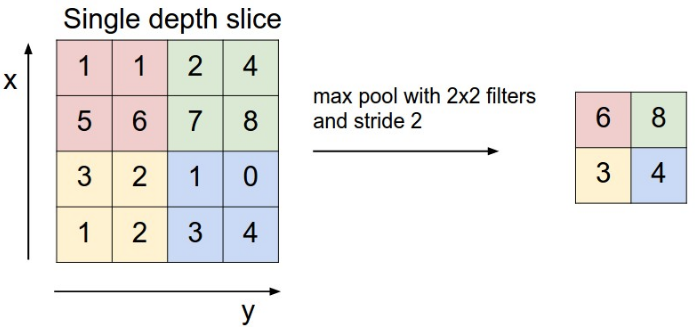
\includegraphics[width=0.75\textwidth]{resources/cnn/pooling.png}
  \caption{
    Max pooling Operation mit $ 2 \times 2 $ Filtern und \gls{stride} 2
    \cite{convnet-demo}
  }
  \label{image:pooling}
\end{figure}

\section{Transposed Convolution}
Im Gegensatz zu einer Pooling Layer ermöglicht eine Transposed Convolutional Layer, die Dimensionen von einem Volumen zu vergrößern.
Die funktionsweise einer Transposed Convolution wird anhand von einem Beispiel erklärt. 
\\
Ausgehend von einer $ 2 \times 2 $ Input Matrix, die auf $ 3 \times 3 $ vergrößert werden soll, ein $ 2 \times 2 $ Filter, 
Null Padding und Stride 1, ergibt sich der folgenden Output. 

\begin{figure}[H]
  \centering
  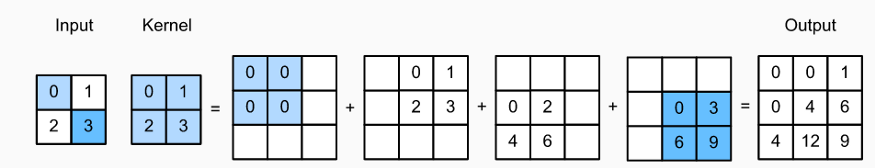
\includegraphics[width=1\textwidth]{resources/cnn/transposed-conv.png}
  \caption{
    Die komplette Transposed Convolution Operation
    \cite{zhang2020dive}
  }
  \label{image:transposed-conv}
\end{figure}

Jede Zahl in der Input Matrix wird mit jeder Zahl in den Filtern multipliziert. Daraus ergibt sich an jeder Position in der Input Matrix einer 
$ 2 \times 2 $ Matrix. Die sich überlappenden Zahlen auf der Output Matrix werden addiert. Daraus ergibt sich eine $ 3 \times 3 $ Output Matrix.

\section{Autoencoder}
Ein Autoencoder ist ein neuronales Netz, welches versucht die Eingangsinformationen zu komprimieren und mit den reduzierten Informationen 
im Ausgang wieder korrekt nachzubilden \cite{was-ist-autoencoder}. Die Komprimierung und Rekonstruktion des Inputs läuft in zwei Schritten ab, 
weshalb das Netz in zwei Teile betrachtet werden kann.
\\
\subsubsection{Encoder}
Der Encoder reduziert die Dimensionen von einem Input und somit werden die wichtigsten Features in einer reduzierter Dimension komprimiert.
In einem neuronalen Netz wird diese Komprimierung durch die Hidden Layers erreicht. Der Encoder ist definiert als:

\begin{equation}
  h = f(x)
\end{equation}

wobei $x$ ein Input ist, $f$ der Encoder und $h$ die Kodierten Features von $x$.

\subsubsection{Decoder}
Der Decoder ist zuständig für die Rekonstruktion von $x$ anhand $h$ und ist definiert als:

\begin{equation}
  \hat{x} = g(h)
\end{equation}

wobei, $\hat{x}$ der rekonstruierte Input ist, $g$ der Decoder und $h$ die Kodierten Features.

In der vorliegenden Arbeit wird eine Variante von Autoencoder, basierend auf Convolutional Neural Networks, eingesetzt.

\section{\textit{Lab}-Farbraum} 
Der \textit{Lab}-Farbraum (auch CIELAB-Farbraum genannt) ist ein Farbraum definiert bei der internationalen
Beleuchtungskommission (\gls{cie}) in 1976. Farben werden mit drei Werten beschrieben. ``\textit{L}'' (Lightness) definiert die Helligkeit.
Die Werte liegen zwischen 0 und 100. ``\textit{a}'' gibt die Farbart und Farbintensität zwischen Grün und Rot an und ``\textit{b}'' gibt die
Farbart und Farbintensität zwischen Blau und Gelb wieder. Die Werte für ``\textit{a}'' und ``\textit{b}'' liegen zwischen -128 und 127.
\\
In der vorliegenden Arbeit wird der \textit{Lab}-Farbraum verwendet, da es unkompliziert ist, den ``\textit{L}'' Kanal von beiden Farbkanälen
``\textit{a}'' und ``\textit{b}'' zu trennen. Außerdem bildet der \textit{Lab}-Farbraum das menschliche Sehvermögen besser ab, als der 
RGB-Farbraum\footnote{RGB steht für Red, Green und Blue, die 3 Farbkanäle des Farbraums}.

\section{Image Colorization Methoden}
Der Prozess von Image Colorization kann manuell oder automatisch erfolgen. Zu den manuellen Methoden zählen die analoge Einfärbung eines Bildes
durch einen Menschen bis hin zur digitalen Bearbeitung mit einem dafür vorgesehenem Programm. Für die automatischen Methoden wird öfters menschlicher Input
benötigt, um zum Beispiel Bereiche von einem Graustufenbild mit Farbstichen zu markieren, die dann automatisch von einem Algorithmus über das Bild
propagiert werden. Aktuelle automatische Methoden nutzen die Vorteile von Convolutional Neural Networks, um diesen Prozess effizienter und performanter
zu gestalten.

Um ein CNN, der Bilder automatisch einfärbt, zu trainieren, werden das Original Bild und das Graustufenbild benötigt. Das Graustufenbild wird
in den CNN eingespeist und dieser wird versuchen die Farbkanal Werte vorherzusagen. Anschließend werden die Werte von jedem Pixel mit jedem Pixel
aus dem Original Bild verglichen. Dieser Prozess wird iterativ wiederholt, bis die erzeugten Werten einen niedrigen Loss Wert haben. In den
nächsten Kapiteln wird dieser Vorgehensweise näher erläutert.

\section{Verwandte Arbeiten}\label{subsection:verwandte-arbeiten}
Vor der Erstellung dieser Arbeit wurden zahlreiche automatische Methoden von Image Colorization bereits untersucht. Frühere Methoden waren
stark an menschliches Input
gebunden. Die Methode von Levin et al. verwendet Farbstiche auf dem Graustufenbild, die automatisch von einem Algorithmus über das gesamte 
Bild propagiert werden \cite{10.1145/1015706.1015780}.
\\
\\
Der Fokus dieser Arbeit ist auf voll automatische Image Colorization Methoden gesetzt. Konservative Methoden, die Convolutional Neural Networks 
verwenden, versuchen die Farben von dem originalen Bild wiederherzustellen, indem die \gls{loss function} die Distanz der vorhergesagten
Farben zu den realen Farben berechnet. Diese Methoden liefern in der Regel entsättigte und blasse Bilder wie bei \cite{zbulak2019image}. 
Einer der Gründe für diese Ergebnisse ist, dass die Modelle nicht richtig lernen. So können beispielsweise Äpfel verschiedene Farben 
wie Rot oder Grün haben. Wenn das Netzwerk mit einem MSE Loss trainiert wird und der Datensatz die gleiche oder annähernd gleiche Anzahl an
grünen und roten Äpfeln hat, wird der Output bei einem Apfel eine Farbe zwischen Rot und Grün sein, was ein entsättigtes Bild erzeugen wird.
\\
\\
Aus diesem Grund betrachtet die vorliegende Arbeit das Problem von Image Colorization als ein Multimodales Problem, 
da gleiche Objekte verschiedene Farben einnehmen können.
Die vorliegende Arbeit orientiert sich an die Methoden von Zhang et al. und Billaut et al., die ähnliche Ansätze für Image Colorization vorschlagen.
Sie betrachten das Problem als ein Klassifizierungsproblem und trainieren eine CNN mit der Cross Entropy und Weighted Cross Entropy Loss. 
Der Output des Netzwerks ist eine Wahrscheinlichkeitsverteilung über die möglichen Bins für jeden Pixel, die im Kapitel \ref{section:binning} erläutert werden.
\\
\\
Beide Ansätze verwenden ``Color \gls{bin}s'' die es unkompliziert ermöglichen die Farben von jedem Pixel zu klassifizieren. 
Es wird im nächsten Kapitel weiter auf diese Methode eingegangen.
